\mode*
\section{The make Utility}

\begin{frame}{make}
  To compile a single C program:
  \begin{itemize}
  \item[\$] \texttt{gcc hello.c -o hello} \tikz \node [opacity=.4,red,scale=3,inner
    sep=0pt,label={[below=2.5ex,right]{\tiny OK. But...}}] {\Checked};
  \end{itemize}
  \begin{block}{What if you have a large project with 1000+ \texttt{.c} files?}
    \begin{center}
      \mode<beamer>{ 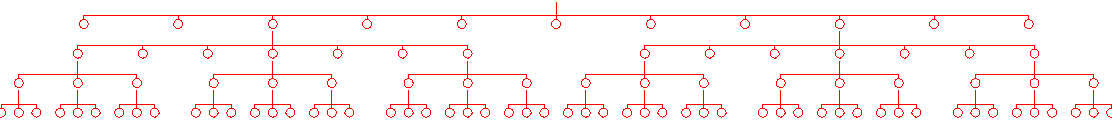
\includegraphics[width=\textwidth]{tree} }%
      \mode<article>{ 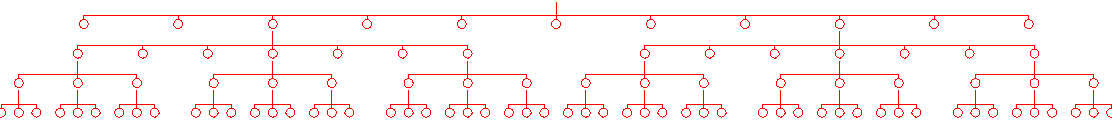
\includegraphics[width=.5\textwidth]{tree} }
    \end{center}
    \begin{description}
    \item[Linux 4.9 source tree:] 3799 directories, 55877 files
    \end{description}
  \end{block}
  \begin{description}
  \item[make:] help you maintain your programs.
  \end{description}
\end{frame}

\begin{frame}{Makefile}
  \begin{block}{}
      \mode<beamer>{ 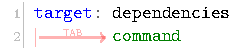
\includegraphics[width=.5\textwidth]{mktab1} }%
      \mode<article>{ 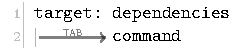
\includegraphics[width=.3\textwidth]{mktab1-bw} }
  \end{block}
  \begin{block}{Example}
      \mode<beamer>{ 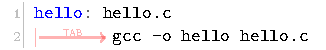
\includegraphics[width=.6\textwidth]{mktab2} }%
      \mode<article>{ 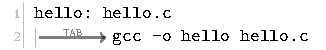
\includegraphics[width=.4\textwidth]{mktab2-bw} }
  \end{block}
  \begin{itemize}
  \item[\$] \texttt{info make makefiles}
  \end{itemize}
\end{frame}

\begin{frame}{Makefile}
  \begin{minipage}{.75\linewidth}
    \mode<beamer>{ 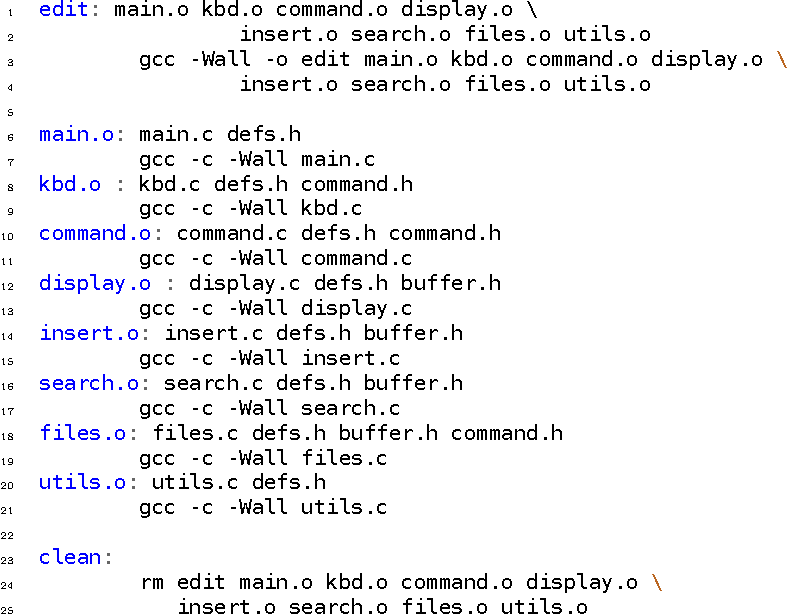
\includegraphics[width=\textwidth]{Makefile2-mk} }%
    \mode<article>{ 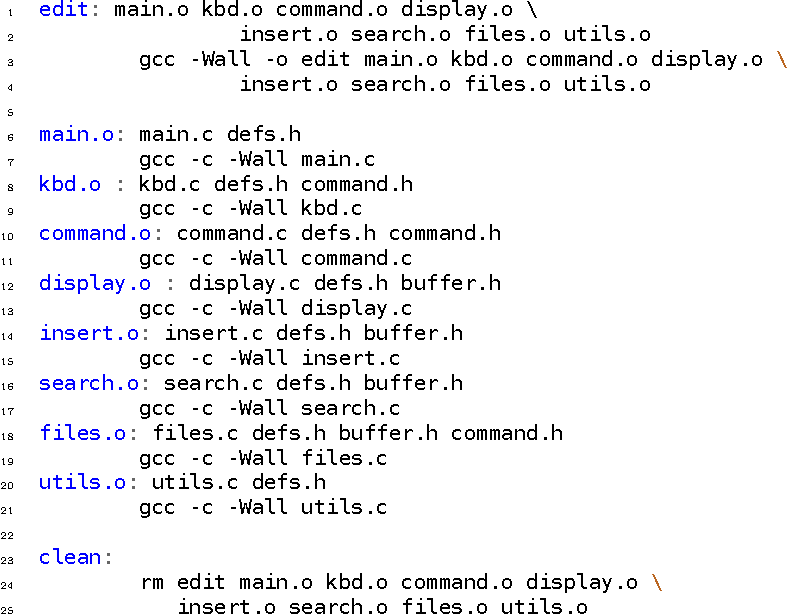
\includegraphics[width=\textwidth]{Makefile2-mk} }
  \end{minipage}
  \begin{minipage}{.2\linewidth}
    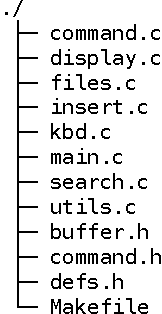
\includegraphics[width=\textwidth]{make-dir-tree}
  \end{minipage}
\end{frame}

\mode<all>
%%% Local Variables:
%%% mode: latex
%%% TeX-master: "c-b"
%%% End:
